\PassOptionsToPackage{unicode=true}{hyperref} % options for packages loaded elsewhere
\PassOptionsToPackage{hyphens}{url}
%
\documentclass[]{article}
\usepackage{lmodern}
\usepackage{amssymb,amsmath}
\usepackage{ifxetex,ifluatex}
\usepackage{fixltx2e} % provides \textsubscript
\usepackage[T1]{fontenc}
\usepackage[utf8]{inputenc}
\usepackage{textcomp} % provides euro and other symbols
% use upquote if available, for straight quotes in verbatim environments
\IfFileExists{upquote.sty}{\usepackage{upquote}}{}
% use microtype if available
\IfFileExists{microtype.sty}{%
\usepackage[]{microtype}
\UseMicrotypeSet[protrusion]{basicmath} % disable protrusion for tt fonts
}{}
\IfFileExists{parskip.sty}{%
\usepackage{parskip}
}{% else
\setlength{\parindent}{0pt}
\setlength{\parskip}{6pt plus 2pt minus 1pt}
}
\usepackage{hyperref}
\hypersetup{
    colorlinks=true,
    linkcolor=blue,
    filecolor=magenta,
    urlcolor=cyan,
}
\urlstyle{same}  % don't use monospace font for urls
\usepackage{color}
\usepackage{fancyvrb}
\newcommand{\VerbBar}{|}
\newcommand{\VERB}{\Verb[commandchars=\\\{\}]}
\DefineVerbatimEnvironment{Highlighting}{Verbatim}{commandchars=\\\{\}}
% Add ',fontsize=\small' for more characters per line
\newenvironment{Shaded}{}{}
\newcommand{\KeywordTok}[1]{\textcolor[rgb]{0.00,0.44,0.13}{\textbf{#1}}}
\newcommand{\DataTypeTok}[1]{\textcolor[rgb]{0.56,0.13,0.00}{#1}}
\newcommand{\DecValTok}[1]{\textcolor[rgb]{0.25,0.63,0.44}{#1}}
\newcommand{\BaseNTok}[1]{\textcolor[rgb]{0.25,0.63,0.44}{#1}}
\newcommand{\FloatTok}[1]{\textcolor[rgb]{0.25,0.63,0.44}{#1}}
\newcommand{\ConstantTok}[1]{\textcolor[rgb]{0.53,0.00,0.00}{#1}}
\newcommand{\CharTok}[1]{\textcolor[rgb]{0.25,0.44,0.63}{#1}}
\newcommand{\SpecialCharTok}[1]{\textcolor[rgb]{0.25,0.44,0.63}{#1}}
\newcommand{\StringTok}[1]{\textcolor[rgb]{0.25,0.44,0.63}{#1}}
\newcommand{\VerbatimStringTok}[1]{\textcolor[rgb]{0.25,0.44,0.63}{#1}}
\newcommand{\SpecialStringTok}[1]{\textcolor[rgb]{0.73,0.40,0.53}{#1}}
\newcommand{\ImportTok}[1]{#1}
\newcommand{\CommentTok}[1]{\textcolor[rgb]{0.38,0.63,0.69}{\textit{#1}}}
\newcommand{\DocumentationTok}[1]{\textcolor[rgb]{0.73,0.13,0.13}{\textit{#1}}}
\newcommand{\AnnotationTok}[1]{\textcolor[rgb]{0.38,0.63,0.69}{\textbf{\textit{#1}}}}
\newcommand{\CommentVarTok}[1]{\textcolor[rgb]{0.38,0.63,0.69}{\textbf{\textit{#1}}}}
\newcommand{\OtherTok}[1]{\textcolor[rgb]{0.00,0.44,0.13}{#1}}
\newcommand{\FunctionTok}[1]{\textcolor[rgb]{0.02,0.16,0.49}{#1}}
\newcommand{\VariableTok}[1]{\textcolor[rgb]{0.10,0.09,0.49}{#1}}
\newcommand{\ControlFlowTok}[1]{\textcolor[rgb]{0.00,0.44,0.13}{\textbf{#1}}}
\newcommand{\OperatorTok}[1]{\textcolor[rgb]{0.40,0.40,0.40}{#1}}
\newcommand{\BuiltInTok}[1]{#1}
\newcommand{\ExtensionTok}[1]{#1}
\newcommand{\PreprocessorTok}[1]{\textcolor[rgb]{0.74,0.48,0.00}{#1}}
\newcommand{\AttributeTok}[1]{\textcolor[rgb]{0.49,0.56,0.16}{#1}}
\newcommand{\RegionMarkerTok}[1]{#1}
\newcommand{\InformationTok}[1]{\textcolor[rgb]{0.38,0.63,0.69}{\textbf{\textit{#1}}}}
\newcommand{\WarningTok}[1]{\textcolor[rgb]{0.38,0.63,0.69}{\textbf{\textit{#1}}}}
\newcommand{\AlertTok}[1]{\textcolor[rgb]{1.00,0.00,0.00}{\textbf{#1}}}
\newcommand{\ErrorTok}[1]{\textcolor[rgb]{1.00,0.00,0.00}{\textbf{#1}}}
\newcommand{\NormalTok}[1]{#1}
\usepackage{longtable,booktabs,multirow}
\usepackage{tabularx}
\newcommand{\ra}[1]{\renewcommand{\arraystretch}{#1}}

% Fix footnotes in tables (requires footnote package)
\IfFileExists{footnote.sty}{\usepackage{footnote}\makesavenoteenv{longtable}}{}
\usepackage{graphicx,grffile}
\graphicspath{{../assets/}{../renderings/}{../schematics/}}
\usepackage{subfig}
\usepackage[page]{appendix}
\makeatletter
\def\maxwidth{\ifdim\Gin@nat@width>\linewidth\linewidth\else\Gin@nat@width\fi}
\def\maxheight{\ifdim\Gin@nat@height>\textheight\textheight\else\Gin@nat@height\fi}
\makeatother
% Scale images if necessary, so that they will not overflow the page
% margins by default, and it is still possible to overwrite the defaults
% using explicit options in \includegraphics[width, height, ...]{}
\setkeys{Gin}{width=\maxwidth,height=\maxheight,keepaspectratio}
\setlength{\emergencystretch}{3em}  % prevent overfull lines
\providecommand{\tightlist}{%
  \setlength{\itemsep}{0pt}\setlength{\parskip}{0pt}}
\setcounter{secnumdepth}{0}
% Redefines (sub)paragraphs to behave more like sections
\ifx\paragraph\undefined\else
\let\oldparagraph\paragraph
\renewcommand{\paragraph}[1]{\oldparagraph{#1}\mbox{}}
\fi
\ifx\subparagraph\undefined\else
\let\oldsubparagraph\subparagraph
\renewcommand{\subparagraph}[1]{\oldsubparagraph{#1}\mbox{}}
\fi

\title{Blue Hunters: Bluetooth RSSI Locator Robots}
\author{Jacob Glueck (\href{mailto:jng55@cornell.edu}{jng55}) \and Jane Du (\href{mailto:zd53@cornell.edu}{zd53}) \and Justin Cray (\href{mailto:jgc232@cornell.edu}{jgc232})}
\date{December 6, 2017}

\begin{document}
\maketitle

\hypertarget{introduction}{%
\subsection{Introduction}\label{introduction}}

Navigating through a plane is a problem with many diverse applications and solutions. We explore the approach of letting a robot use the strength of a broadcasted signal to locate itself. In particular, we investigate using the Received Signal Strength Indicator (RSSI) of Bluetooth Low Energy (BLE) 4.0 chips to allow wheeled mobile robots to navigate towards a stationary base station. The robot detects its proximity to the station based on the strength of the signal and moves towards what it believes to be the signal source. 

In the process of designing and building the hunting robots and the beacon, we encountered an interesting challenge in particular: fake Bluetooth modules from non-official vendors with usable hardware but out-of-date (and poorly documented) firmware. We explain the process we used to find, flash, and verify the correct firmware in order to use it for our project.

Each robot was controlled by a PIC32MX250 microcontroller, and used a 3 axis magnetometer as as compass in order to reliably turn, as well as 2 micro 9 g servos to drive.
Each unit was powered with 3 AA batteries.
Finally, the chassis and wheels of each car were 3D printed.
Figure \ref{fig:robotsystem} shows the entire system.

\begin{figure}
  \centering
  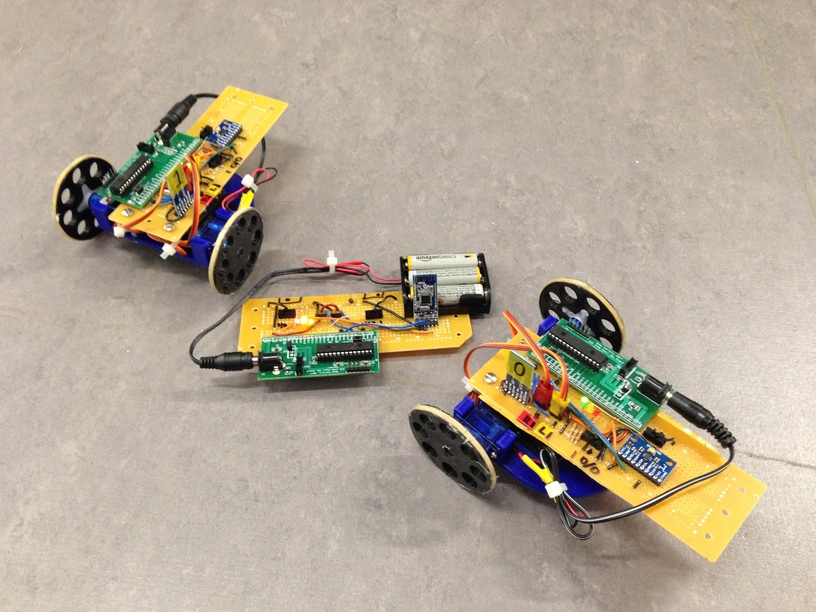
\includegraphics[width=0.8\textwidth]{full_system.jpg}
  \caption{Full system with 2 robots and the base station}
  \label{fig:robotsystem}
\end{figure}

\subsection{Design}

The design of the robots and beacon can be split into 3 rough categories: first, the construction of the robot itself, including the design of the chassis; second, the integration of the bluetooth modules that were used to transmit and receive signals, and lastly, the algorithm and sensors used by the robot to orient itself and move towards the source of the signal.

\subsubsection{Robot Construction}

The system consists of 2 robots, and a base station.
We designed the robots to be small, light, and maneuverable.
Each robot has 2 wheels, driven by a 9 gram micro servo, as well as a third round plastic leg, serving as a caster wheel.
We 3D printed the robot's frame in ABS, resulting in an easy to assemble robot.
After printing the parts, we mounted a 3 AA battery pack to the frame to provide power,
and screwed in a perfboard on standoffs. See \ref{fig:robotchassis} for the parts in each robot.

\begin{figure}
  \centering
  \subfloat[Frame] {
    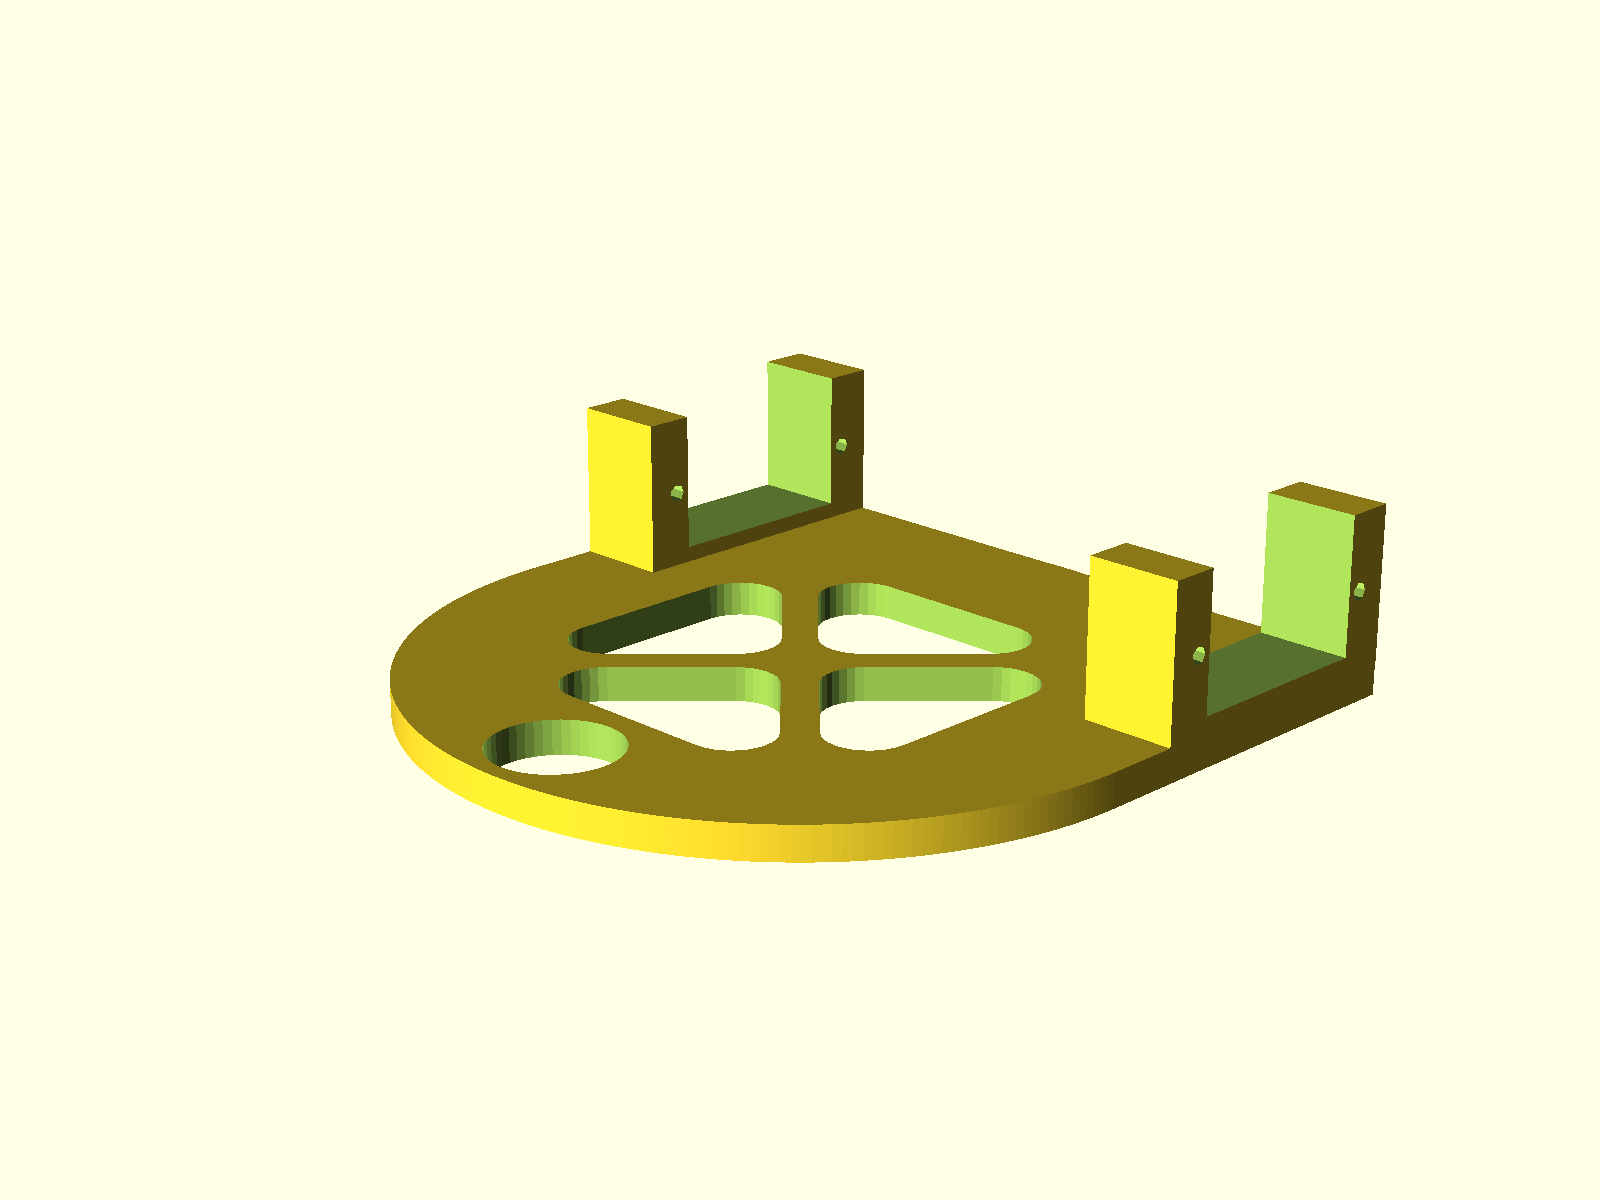
\includegraphics[width=0.4\textwidth,height=\textheight]{frame.png}
    \label{fig:robotfrane}
  }
  \subfloat[Wheel]{
    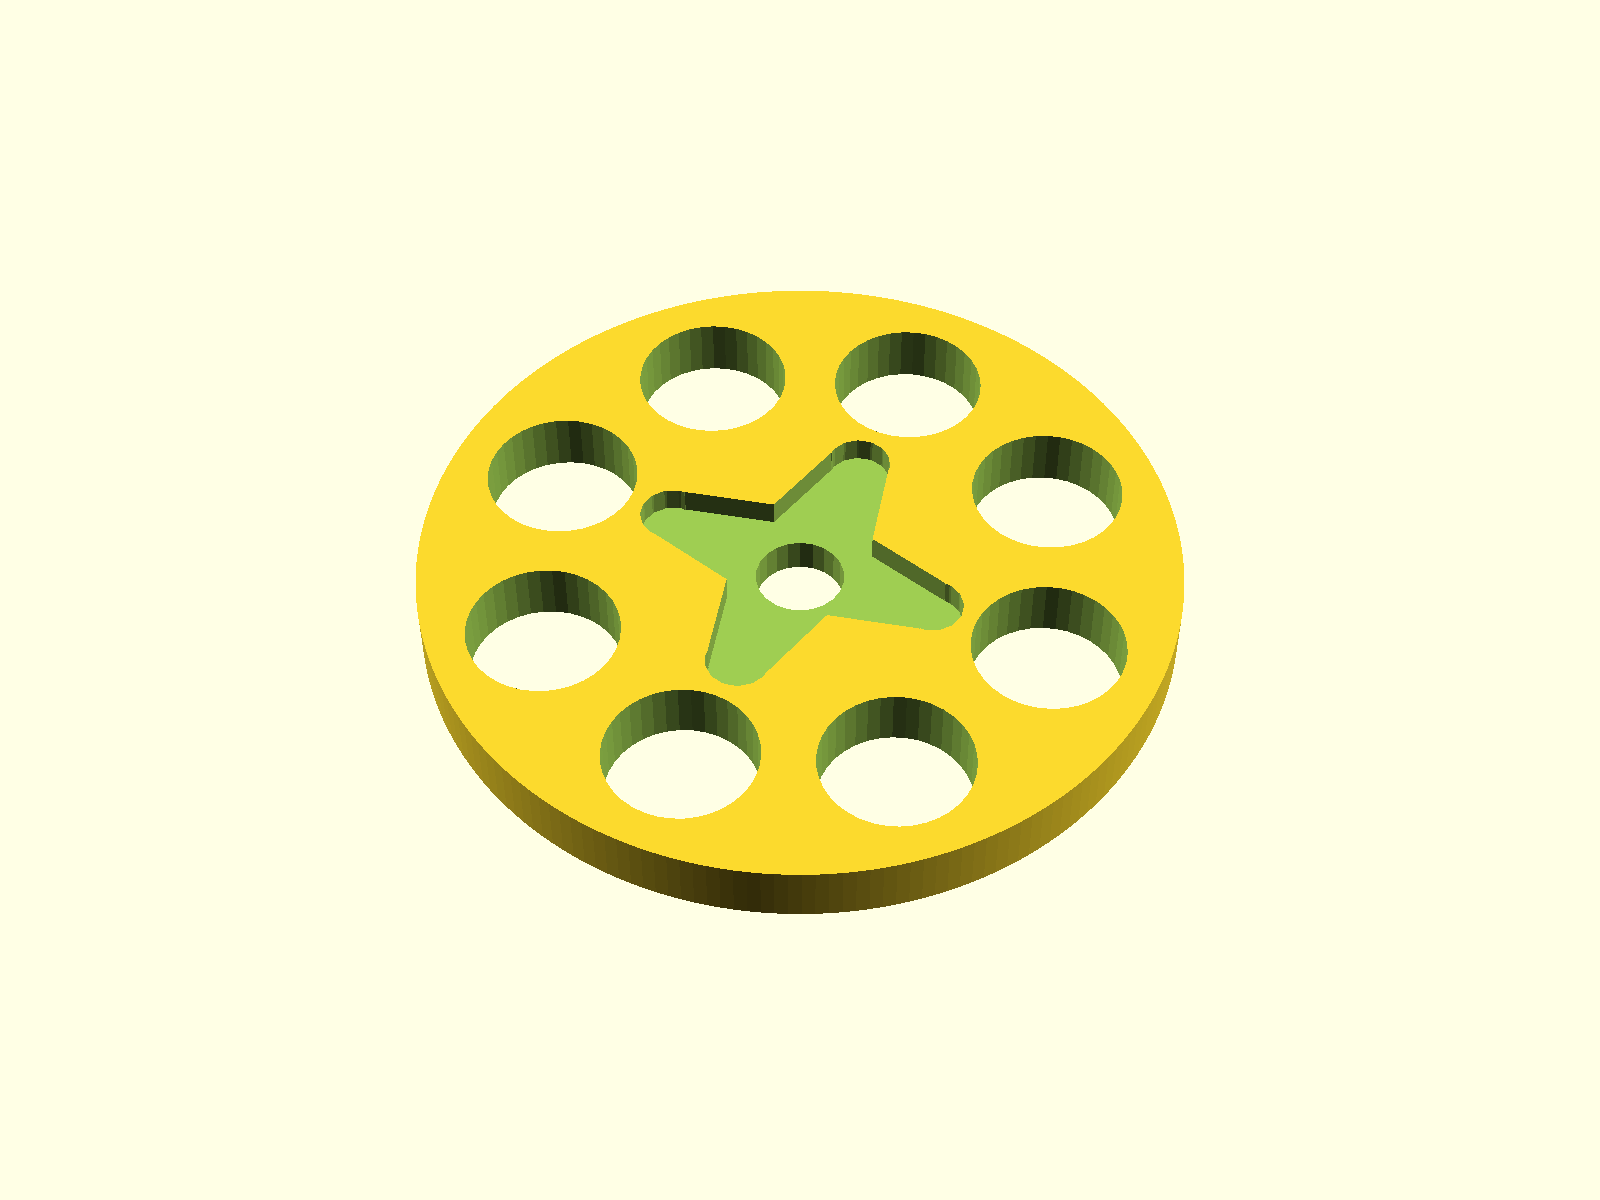
\includegraphics[width=0.4\textwidth,height=\textheight]{wheel.png}
    \label{fig:robotwheel}
  }
  \\
  \subfloat[Caster]{
    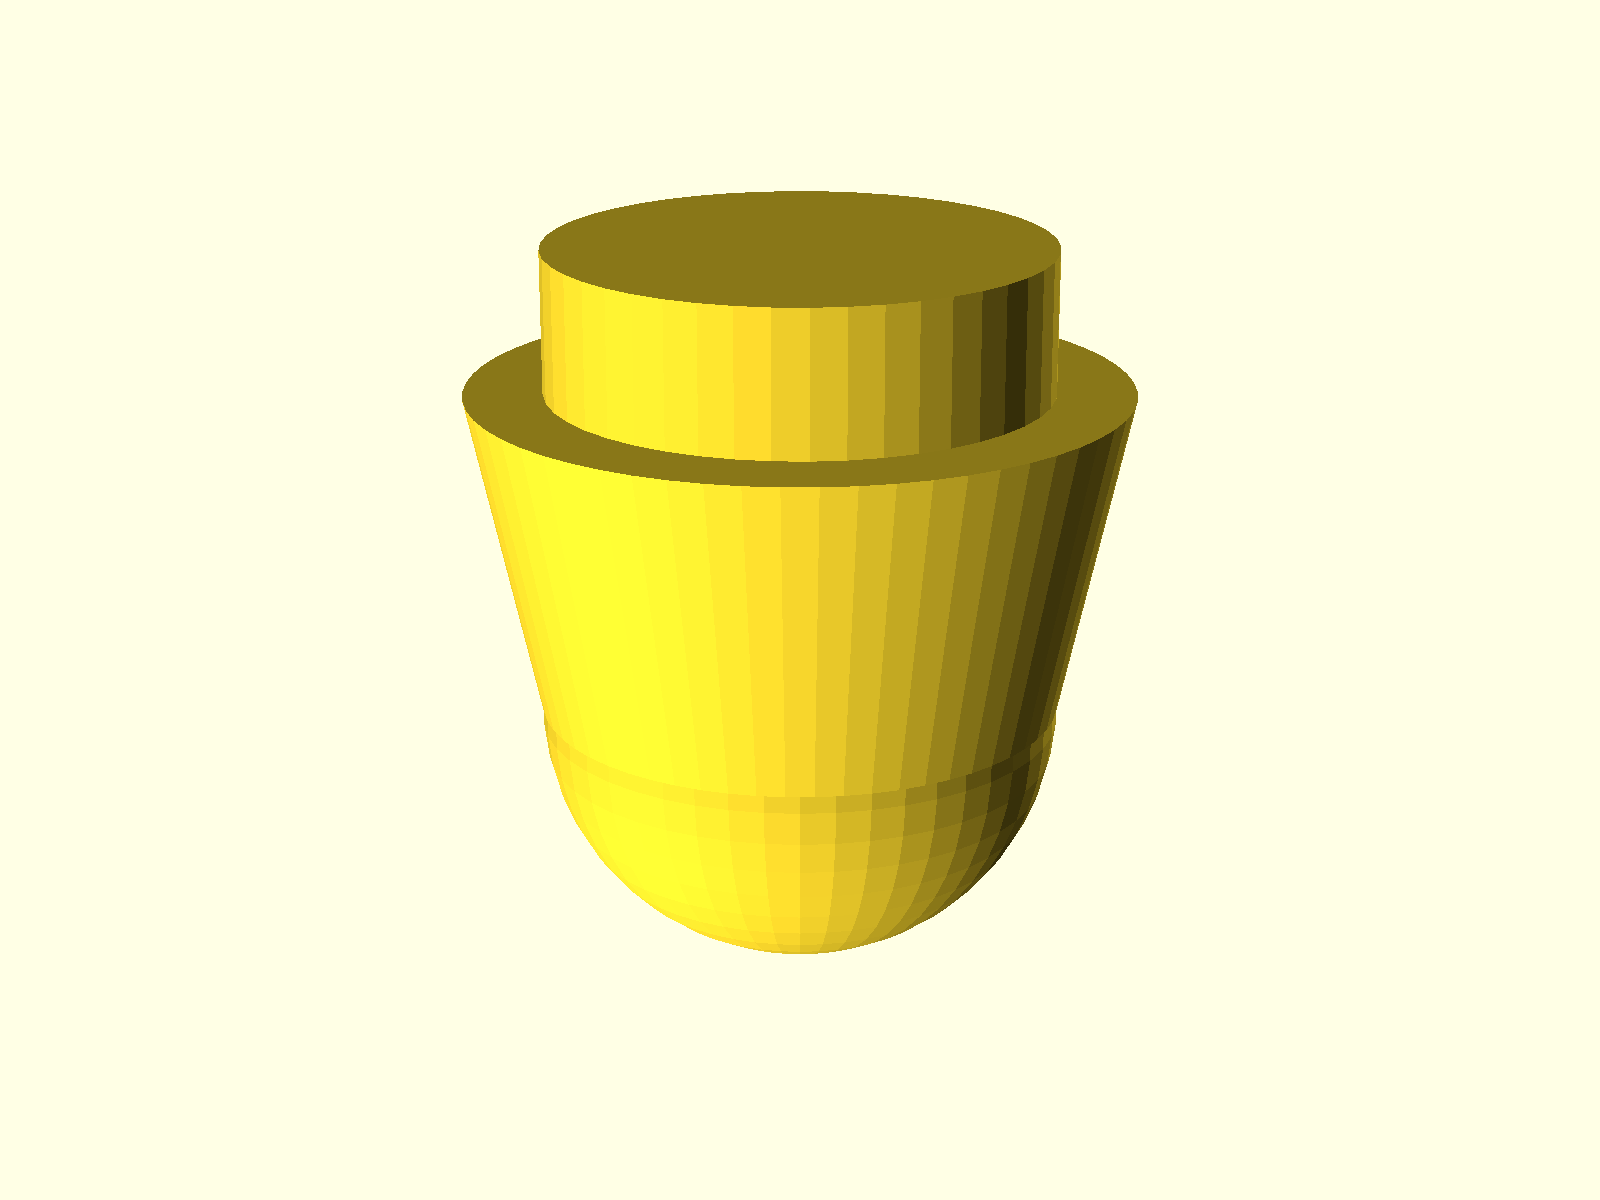
\includegraphics[width=0.4\textwidth,height=\textheight]{drag.png}
    \label{fig:robotcaster}
  }
  \caption{Components of robot chassis}
  \label{fig:robotchassis}
\end{figure}

The electronics for each robot consisted of 4 main components: a PIC32MC250F128B microcontroller, a MPU-9250 IMU with a 3 axis gryoscope, accelerometer, and magnetometer, a HM-10 BLE module with a Texas Instruments CC2541 chip, and two 9 gram FS90R micro continuous rotation servos.
The BLE module connected to the PIC through a UART connection, and the IMU connected to the PIC through an I2C bus.
The base station was identical to the robots, minus the IMU and servos.
The HM-10 Bluetooth module was mounted perpendicular to the breadboard, sticking up in the air to hopefully improve the performance of the radio. Figure \ref{fig:schematic} provides a full schematic for one of the robots.

\begin{figure}
  \centering
  \subfloat[] {
    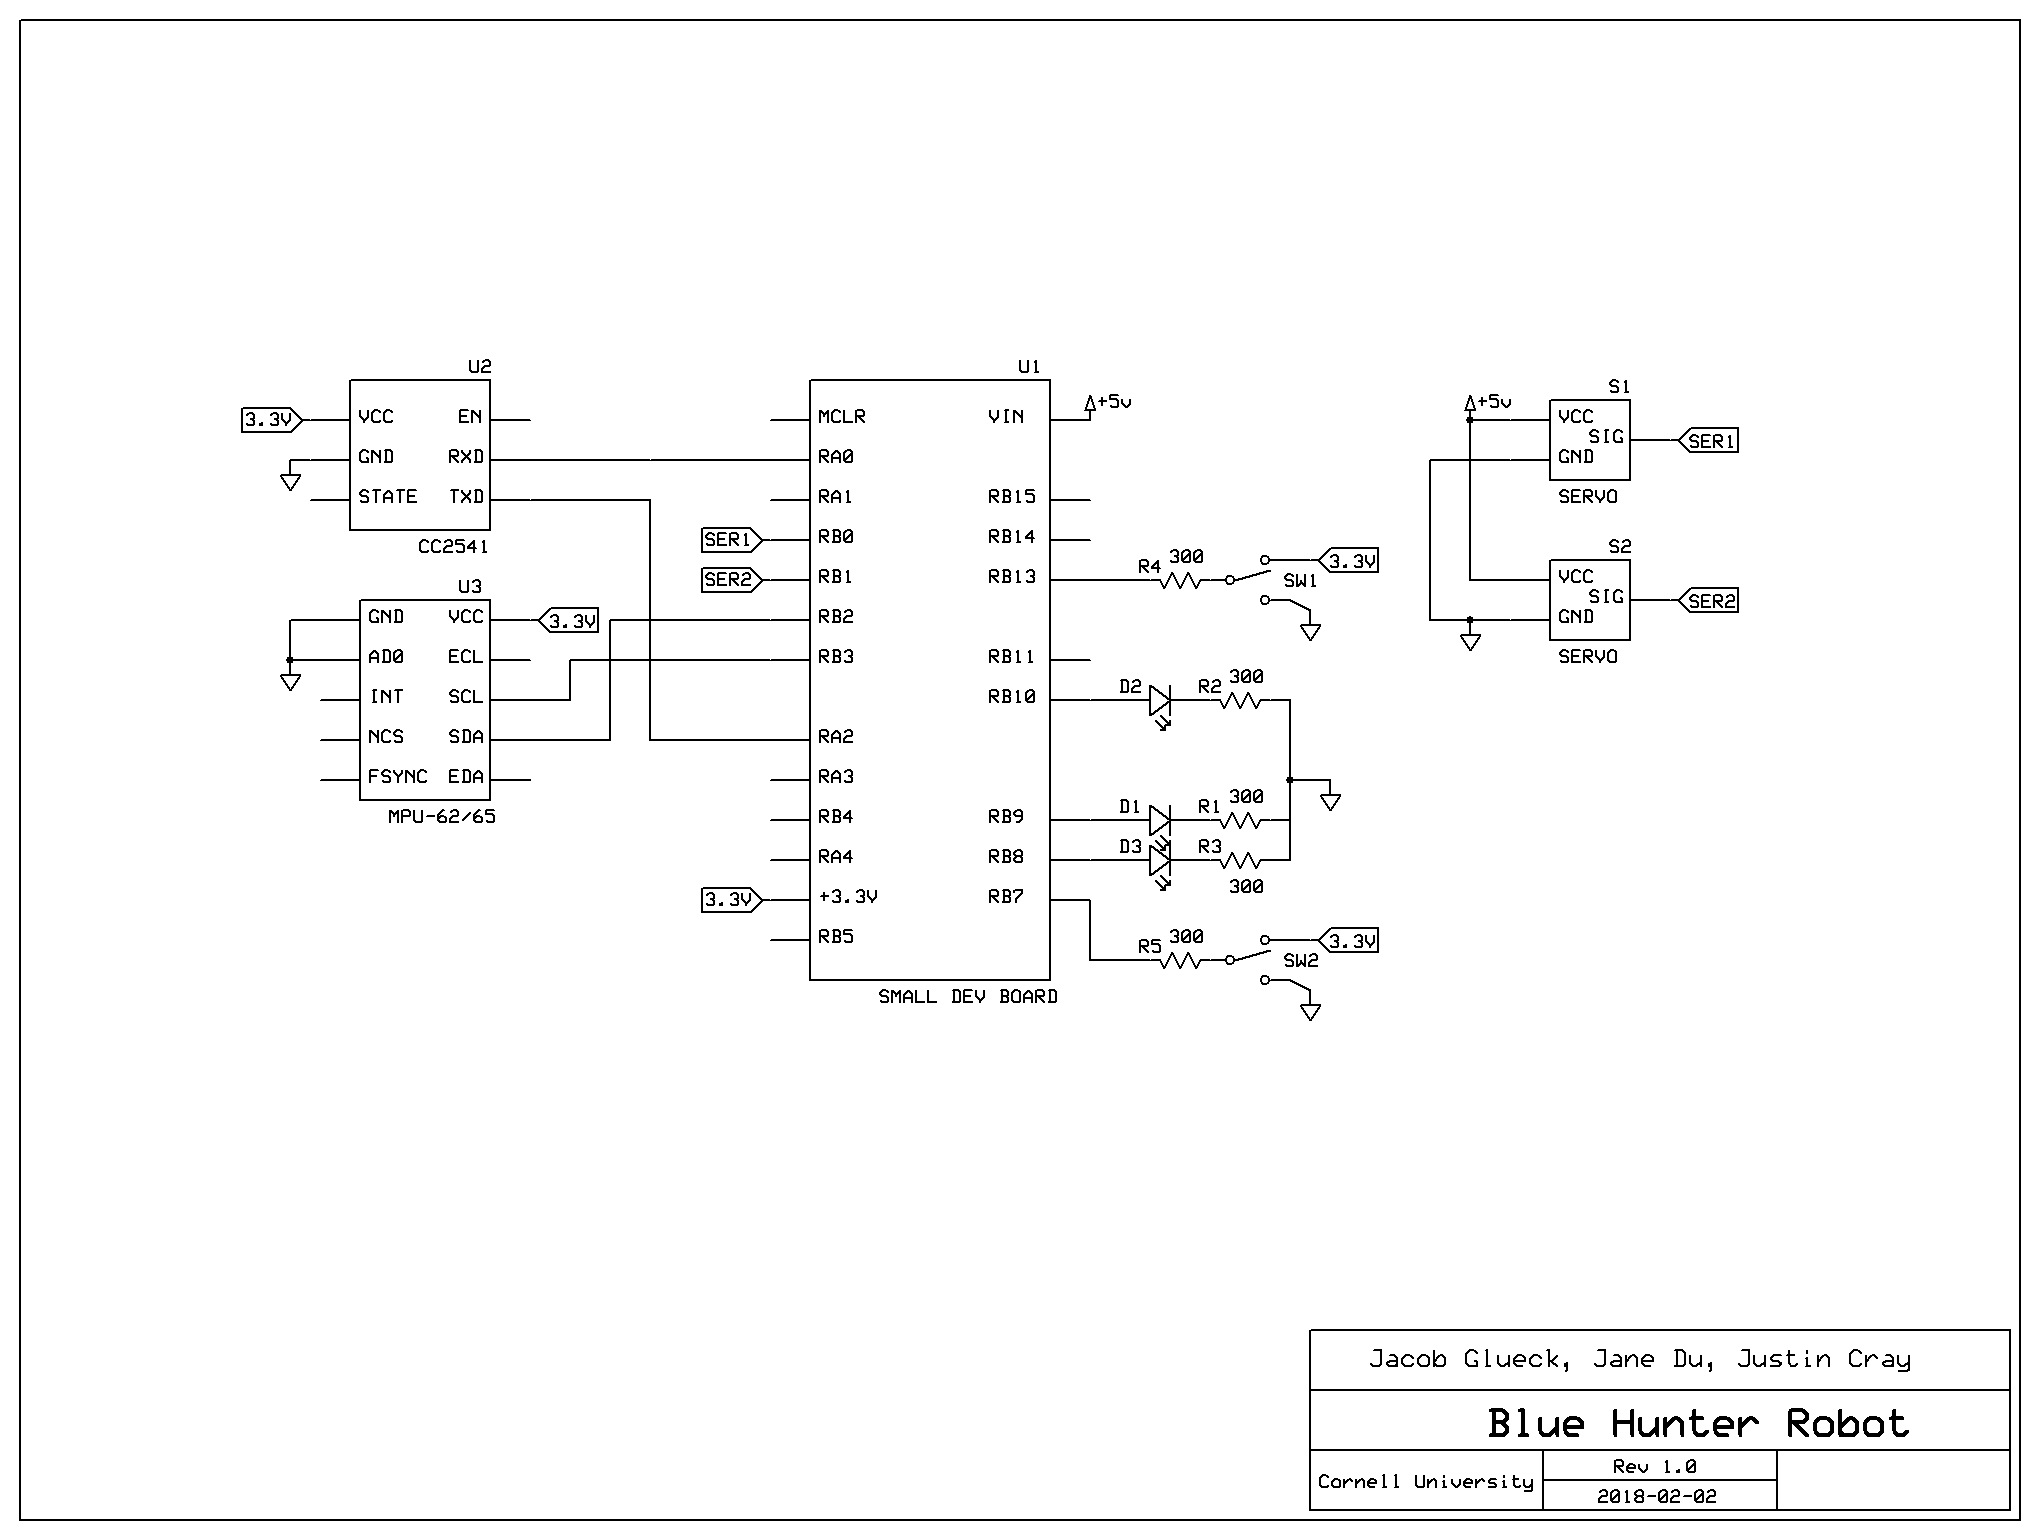
\includegraphics[width=0.9\textwidth]{bluehunters-robot.png}
    \label{fig:schematic-robot}
  }
  \\
  \subfloat[] {
    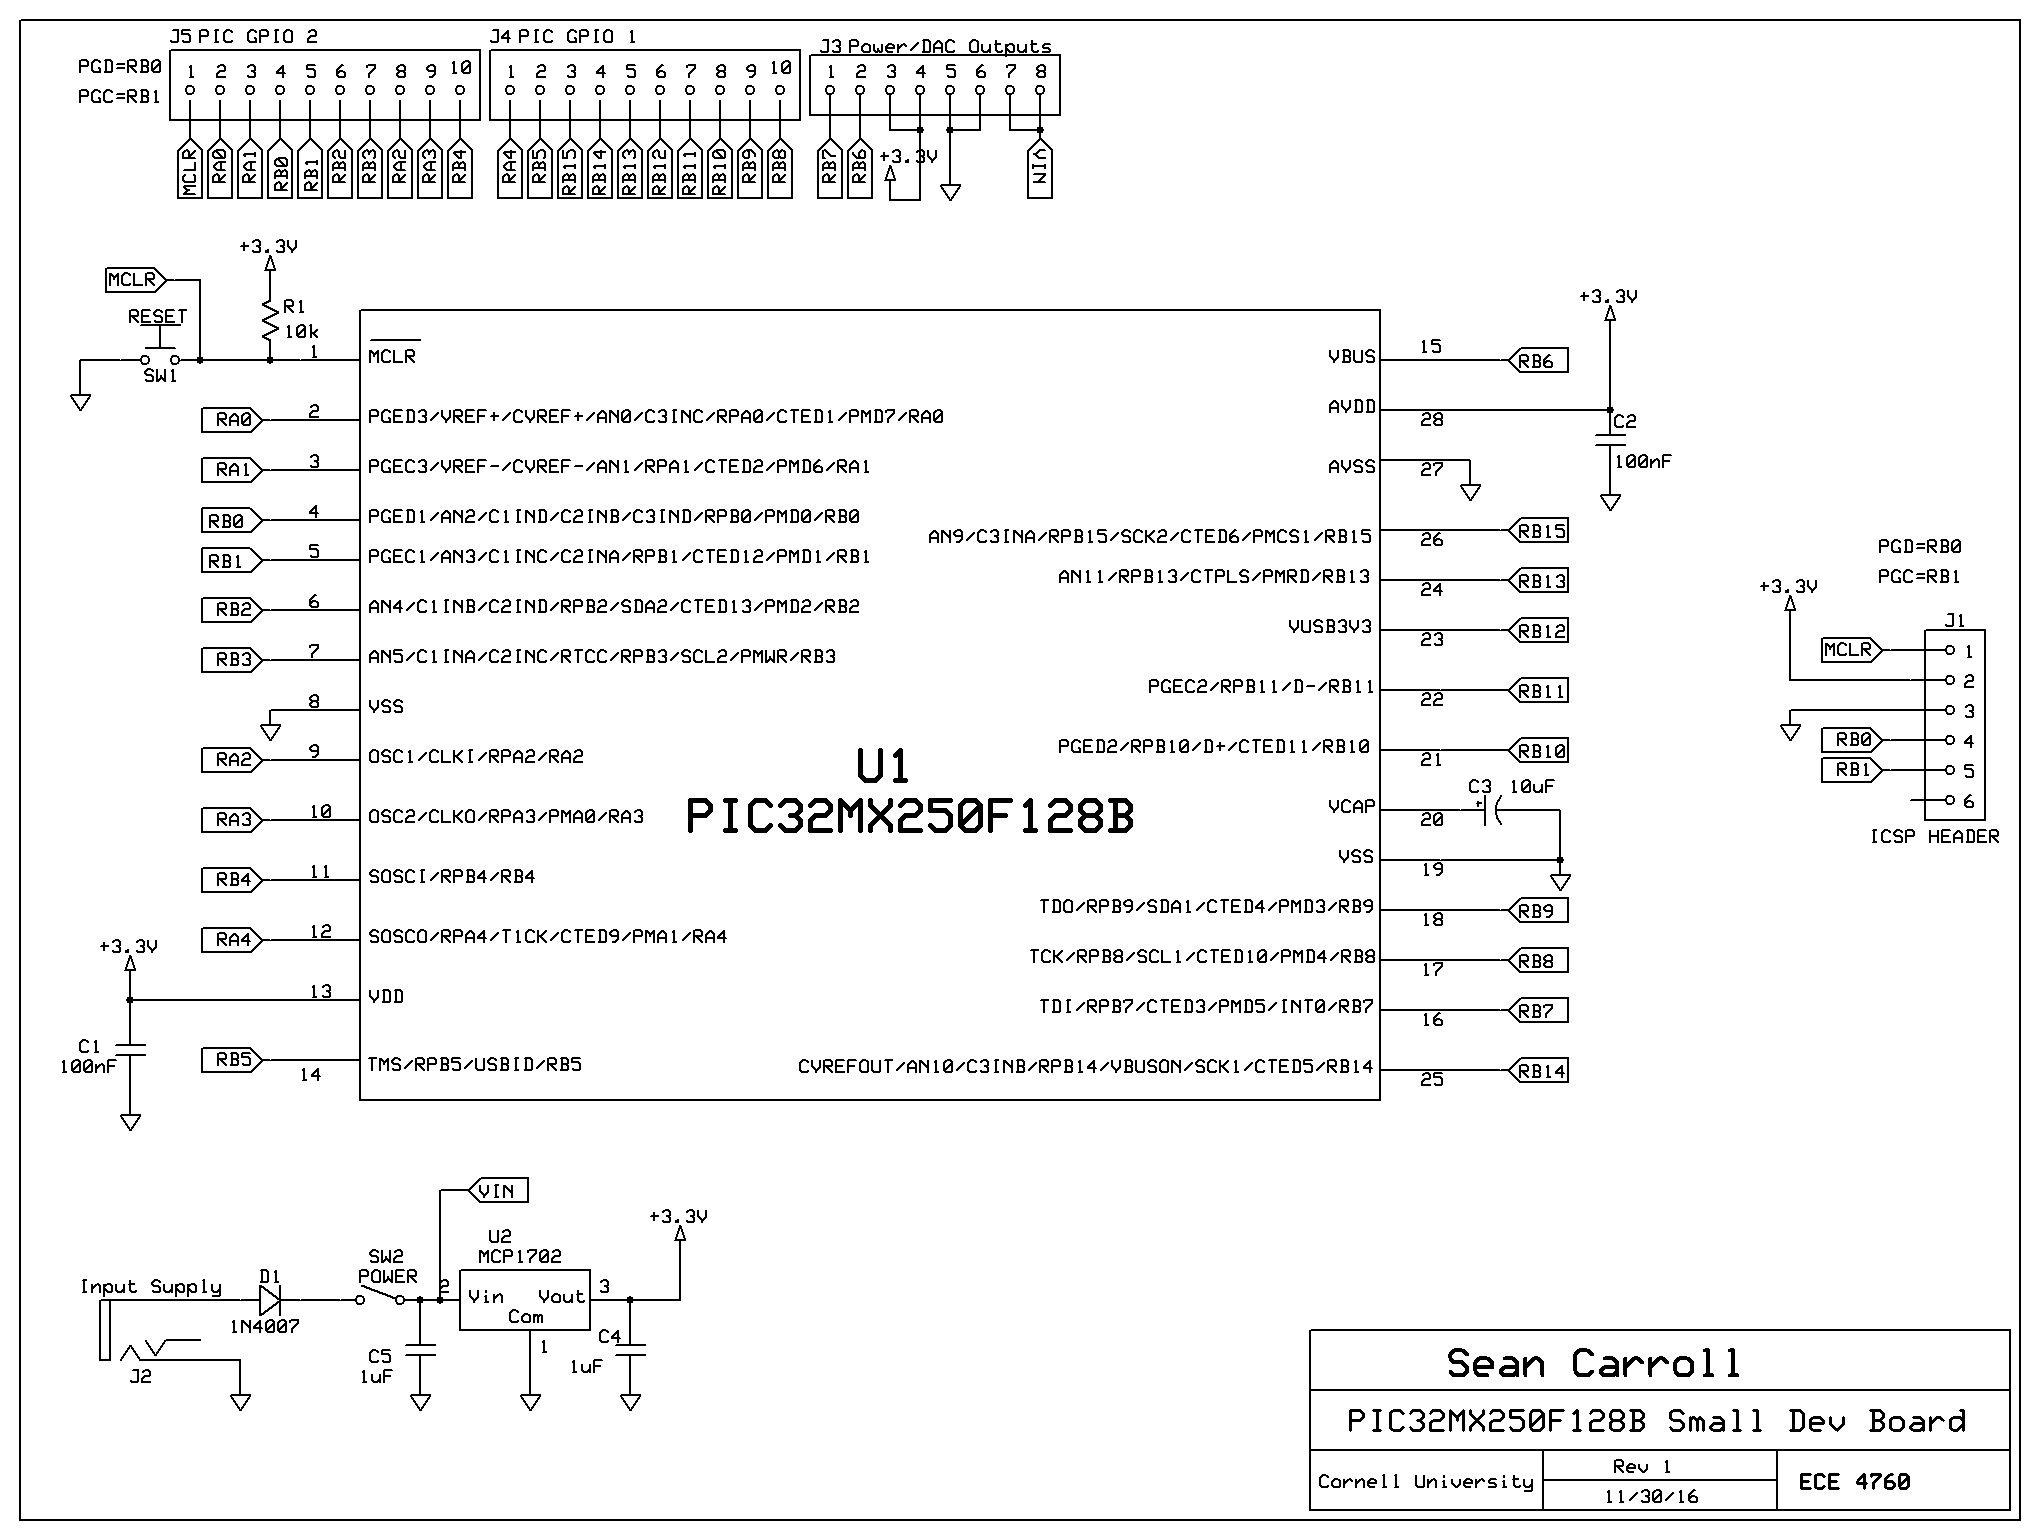
\includegraphics[width=0.9\textwidth]{bluehunters-sdb.png}
    \label{fig:schematic-sdb}
  }
  \caption{Schematic}
  \label{fig:schematic}
\end{figure}

While trying to use the Bluetooth modules (which we bought off Ebay), we discovered that they didn't adhere to the data sheet \cite{jnhuamaodatasheet}, and after doing some research, concluded they were fake!
While the boards still had TI CC2541 chips, the firmware they were running was not the genuine Jnhuamao firmware.
Luckily, the only difference between the fake boards and the genuine boards was that then genuine boards had an external crystal, but the genuine firmware checks for the presence of the crystal, and works even without it. \cite{crystal}
Because of that, we were able to salvage the fake chips by reprogramming them with genuine firmware according to an Arduino Fourm post \cite{crystal}.
Essentially, we connected the fake chips to an Arduino Teensy (which is 3.3 volts, and so won't damage the 3.3 volt CC2541) as indicated in table \ref{table:progpins}, using the schematic in figure \ref{fig:hm10} for reference.

\begin{table}[]
  \centering
  \begin{tabular}{@{}lll@{}}
    \toprule
    Name & CC2541 Pin & Arduino Pin\tabularnewline
    \midrule
    \texttt{DEBUG\_CLOCK} & 7 & 5\tabularnewline
    \texttt{DEBUG\_DATA} & 8 & 6\tabularnewline
    \texttt{RESET\_N} & 11 & 4\tabularnewline
    \bottomrule
  \end{tabular}
  \caption{Arduino to CC2541 pin connections for programming.}
  \label{table:progpins}
\end{table}

\begin{figure}
  \centering
  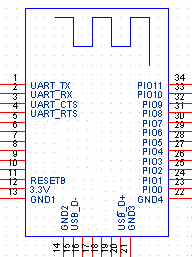
\includegraphics[width=0.3\textwidth]{hm10_pins.png}
  \caption{HM-10 module pin layout \cite{crystal}}
  \label{fig:hm10}
\end{figure}

Then, we uploaded the \texttt{CCLoader.ino} \cite{ccloader} sketch to the Arduino.
This sketch bit bangs the programming signals for the CC2541/
Finally, we ran (in a Windows virtual machine, due to the dubious origin of the software) \texttt{CCLoader.exe} \cite{ccloaderexe}:
\begin{Verbatim}[gobble=2]
  CCLoader.exe <COM Port> <Firmware.bin> 0
\end{Verbatim}
The firmware file came from the Arduino forum post. \cite{firmwarefile}

Next, we updated the chips firmware from from 540, the version we just flashed onto it, to the latest (at the time we did this project) released version, 603. \cite{jnhuamao603}
We connected the HM-10 module to a computer using a 3.3 V FTDI to USB adapter.
Then, using PUTTY established a serial connection (9600 baud, 8N1) and sent the chip \texttt{AT}. If it is connected properly, it will respond with \texttt{OK}.
Next, send the chip \texttt{AT+SBLUP} to put it in firmware update mode.
It will respond with \texttt{OK+SBLUP}. Terminate the PUTTY session.
Run the \texttt{HMSoft.exe} program distributed in the firmware update download.
(Again in a Windows virtual machine, due to the dubious origin of the software.)
Select the proper port and firmware file using the software, and hit ``Load Image''.
The software should handle the rest!
To make sure it worked, establish a serial connection again using PUTTY.
Send \texttt{AT+VERS?} to query the chip for version information.

% \cite{jnhuamaoinstructions}

At this point, we finally had the bluetooth chips in a working state.
In order to have them measure signal strength, we sent it the sequence of commands
shown in table \ref{table:blecommands} in order to obtain a signal strength measurement.
One interesting thing to note about the chip is that commands do not have to end with newlines or carriage returns.
However, if sent, the chip will ignore them.

\begin{table}[]
\centering
\ra{1.3}
\caption{HM-10 Bluetooth module signal strength measurement commands}
\label{table:blecommands}
\begin{tabularx}{\textwidth}{@{}l X@{}}
\toprule
Command & Description \\ \midrule
\texttt{AT+RESET} & Resets the chip to ensure it is in a clean state
before receiving other commands. \\

\texttt{AT+IBEA1} & Sets the iBeacon functionality of the chip (1 on, 0 off).
This allows the chip to be found with an RSSI scan. \\

\texttt{AT+ROLE\{0|1\}} & Sets the role to either peripheral (0) or central (1).
The base station is set to peripheral, and the 2 robots are set to central.
Peripheral means the device will respond in inquiries from a central device.
This allows it to be discovered during an RSSI scan.\\

\texttt{AT+IMME\{0|1\}} & Sets the work state of the device to either actively
listening for Bluetooth signals (0), or only acting when it receives a serial
command (1). Once again, the base station is set to 0: it needs to listen for
signals and respond. The robots are set to 1, as the chips need to initiate scan
requests when they receive the command over serial. \\

\texttt{AT+NAME\{str\}} & Sets the name of the chip (which is visible when
scanning) to the string \texttt{str} (For example, \texttt{AT+NAMEPIRATE} names
the chip \texttt{PIRATE}). We give all the chips unique names to make
debugging easier. \\

\texttt{AT+SHOW3} & Configures the device to advertise both its name
and RSSI when scanning. \\

\texttt{AT+ADDR?} & Queries the device for its hardware address. We
recorded the hardware device of each chip, as when doing RSSI scans,
the results are reported by hardware address. \\

\texttt{AT+DISI?} & Performed only on the robots, causing a discovery
scan. The result of the scan is a series of lines of the form:
{\begin{align*}
&\mathtt{OK+DISC:00000000:00000000000000000000000000000000:}\\
&\mathtt{  0000000000:6832A3801EBE:-080}
\end{align*}}
The second to last token, \texttt{6832A3801EBE}, is the hardware
address of the discovered device, and the last token, \texttt{-080},
is the measured RSSI. The chip will transmit a line for each device it
finds (``line'' is a misnomer as it does not separate them with any
characters), followed by \texttt{OK+DISCE}. \\
\bottomrule
\end{tabularx}
\end{table}

Once we had the Bluetooth signal strength working, we configured the IMU,
a QFN MPU-9250 \cite{mpu9250datasheet} \cite{mpu9250regmap} module.
It has 2 dies: one is the AK8963 3-axis magnetometer \cite{ak8963cdatasheet},
and the other contains the 3-axis gyroscope and 3-axis accelerometer, which we did not use.

The microcontroller communicates with the IMU via I2C, and the compass is connected to the rest of the MPU module via an auxiliary I2C bus. For communication between the microcontroller and the AK8963's main die, we based our work off of basic I2C functions from another ECE 4760 project, the Self-Balancing Robot \cite{selfbalancingrobot}. In particular, their \texttt{i2c\_helper.h} was very helpful.

For communication with the actual magnetometer, we needed to configure the IMU to set the compass must as a slave on the I2C bus. For this, it was necessary to enable pass-through mode on the IMU during its configuration.

The AK8963 has several modes of operation, and the chip must be set to power-down mode before switching to other modes.
We read compass values with single measurement mode, as in figure \ref{fig:imu_single_measurement}.

A single compass read involves setting the compass to single measurement mode in 14 bit resolution, reading the 6 data registers (X low, X high, Y low, Y high, Z low, Z high), reading the Status 2 register to check for magnetic sensor overflow (without reading this register, the read is not considered complete and further reads will fail), and finally waiting to ensure that the IMU is not read too frequently, in which case it will not have enough time to take measurements.

\begin{figure}
  \centering
  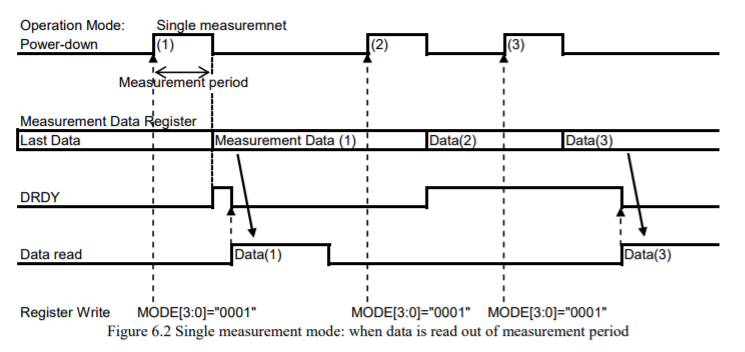
\includegraphics[width=0.9\textwidth]{imu_single_measurement.png}
  \caption{IMU single measurement mode}
  \label{fig:imu_single_measurement}
\end{figure}

In order to calibrate the compass, the robots spun in place when powered
on. They recorded the maximum and minimum values for each axes, and used
that data to scale and center the magnetometer readings.

\subsubsection{Navigation}

Once we had the robots working, we turned to the algorithm.
Since they don't have much data -- only the last couple signal strength measurements --
we decided to use a simple gradient descent algorithm.
Figure \ref{fig:graddesc} shows 2 versions of the gradient descent algorithm.

\begin{figure}
  \centering
  \subfloat[Simple gradient descent]{
    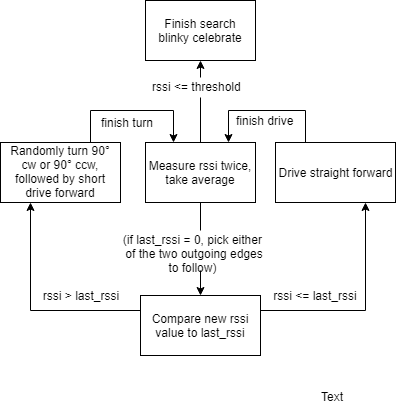
\includegraphics[width=0.4\textwidth]{grad_desc.png}
    \label{fig:simplegrad}
  }
  \subfloat[Compensating gradient descent]{
      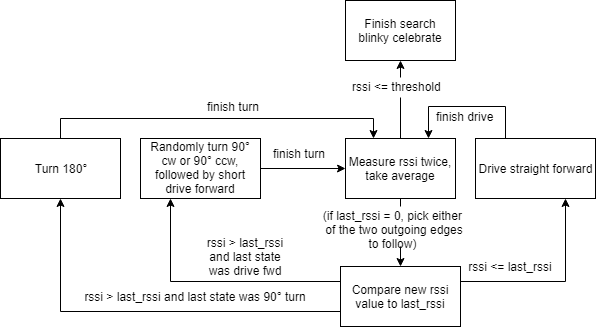
\includegraphics[width=0.5\textwidth]{turn_correction.png}
    \label{fig:compensatinggrad}
  }
  \caption{2 gradient descent algorithms. The initial state is \emph{measure RSSI twice, take average}.}
  \label{fig:graddesc}
\end{figure}

The purpose of the compensating algorithm (figure \ref{fig:compensatinggrad}) was to allow the robots to recover faster after taking a wrong turn: if a robot just just moved forward and detected a weaker signal, turned, and still detected a weaker signal, then it must have turned the wrong way, so it does a 180.
However, it did not prove any more accurate than randomized gradient descent, largely due to noisy RSSI readings.
As such, we used the simplified version.

\subsection{Results}

On average, when starting from 1 meter away, the robots successfully made it to the base station 80\% of the time,
within an average time of 126 seconds.
This wasn't as reliable, or as fast, as we initially hoped.
One of the main reasons for this was the noise in RSSI measurements.

We expected that RSSI would vary with distance according to equation \ref{eq:rssi}:
\begin{equation} \label{eq:rssi}
  \text{RSSI} = A - 10 n \log(d),
\end{equation}
where $A$ and $n$ are RF propagation parameters in dBm, $d$ is distance in meters, and RSSI is the measured RSSI in dBm. \cite{5415423}
We experimented with RSSI measurements to determine how well they worked by taking 2 Bluetooth modules, and measuring the RSSI while moving them apart.
One remained stationary on the floor and the other was moved away from it 1 foot at a time.
At each point, we took 3 RSSI measurements and averaged them. Figure \ref{fig:rssiplot} shows the results (the original data is in table \ref{table:rssidata}).

\begin{figure}
  \centering
  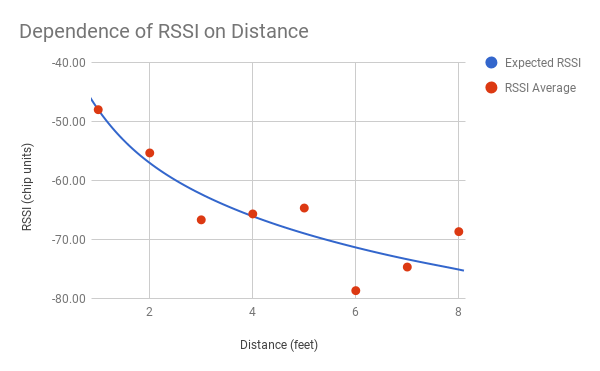
\includegraphics[width=0.9\textwidth]{rssi-chart.png}
  \caption{Plot showing bluetooth RSSI as a function of distance}
  \label{fig:rssiplot}
\end{figure}

\begin{table}
  \centering
  \begin{tabular}[]{@{}llllll@{}}
  \toprule
  Distance (feet) & RSSI A & RSSI B & RSSI C & RSSI Average & Expected
  RSSI \\
  \midrule
  1 & -48 & -48 & -48 & -48.00 & -48.00 \\
  2 & -56 & -58 & -52 & -55.33 & -57.03 \\
  3 & -66 & -66 & -68 & -66.67 & -62.31 \\
  4 & -64 & -68 & -65 & -65.67 & -66.06 \\
  5 & -60 & -70 & -64 & -64.67 & -68.97 \\
  6 & -80 & -80 & -76 & -78.67 & -71.34 \\
  7 & -80 & -79 & -65 & -74.67 & -73.35 \\
  8 & -68 & -66 & -72 & -68.67 & -75.09 \\
  \bottomrule
  \end{tabular}
  \caption{RSSI and distance data}
  \label{table:rssidata}
\end{table}

\begin{table}[]
\centering
\ra{1.3}
\caption{Convergence performance of the robots}
\label{table:convergence}
\begin{tabular}{@{}lllllll@{}}
\toprule
\multirow{2}{*}{Trial} & \multicolumn{3}{c}{Robot 0}       & \multicolumn{3}{c}{Robot 1}      \\ \cmidrule(l){2-4} \cmidrule(l){5-7}
                       & Time (s)  & Distance (cm) & Start & Time (s) & Distance (cm) & Start \\ \midrule
1                      & 213       & 53            & South & 94       & 22            & North \\
2                      & \emph{Timeout} & 420           & South & 153      & 36            & North \\
3                      & 308       & 19            & South & 105      & 36            & North \\
4                      & \emph{Collision} & 340           & South & 80       & 20            & North \\
5                      & \emph{Collision} & 240           & South & 92       & 30            & North \\
6                      & 179       & 46            & North & 117      & 20            & South \\
7                      & 56        & 45            & North & 162      & 24            & South \\
8                      & 59        & 27            & North & 197      & 26            & South \\
9                      & 59        & 19            & North & 79       & 30            & South \\
10                     & \emph{Collision} & 231           & North & 67       & 23            & South \\ \bottomrule
\end{tabular}
\end{table}

\begin{table}[]
\centering
\ra{1.3}
\caption{Average convergence behavior}
\label{table:averagecon}
\begin{tabular}{@{}lll@{}}
\toprule
                       & Robot 0        & Robot 1     \\ \midrule
Convergence time (s)   & 146            & 115         \\
Convergence rate       & 60 \%          & 100 \%      \\
Final distance (cm)    & 35             & 27          \\
Failure distance (cm)  & 308            & --          \\ \bottomrule
\end{tabular}
\end{table}

While the chip reported RSSI in units proportional to dBm, and we
measured distances in feet, not meters, we could still use the above
formula without worrying about unit conversions. The constants $A$ and
$n$, provided we determined them empirically based on the data, would
encode the conversions. As such, we fit the data using the above formula
with $A=-48$ and $n=3$, resulting in the blue curve above. While the
general shape of the curve matches, there is significant noise in the
averaged RSSI data. Furthermore, when we tried to reproduce the
measurements, we could not do so precisely -- it seemed to even depend
on where our feet where!

Despite the noise in the RSSI readings, the robots did surprisingly well.
We tested the robots by starting the both 1 meter from the base station,
one on the north side, and one on the south side.
After they started, we timed the amount of time it took them to arrive
at the base station and flash their LEDs.
We set a timeout of 5 minutes, at which point we would measure the
distance between the robot and the base station.
We also measured the distance when the robot arrived.
All distances were measured between the Bluetooth modules.
The results of this are displayed in table \ref{table:convergence},
with averages in table \ref{table:averagecon}.

There are some interesting patterns in the data.
One obvious one is that robot 1 always made it,
while robot 0 only had a 60\% success rate.
In addition, when robot 1 made it, it was on average 8 centimeters
closer than robot 0, and converged about 30 seconds faster!
We think that perhaps the antennas on each had different sensitivities,
as both used the same RSSI threshold for stopping once they reached the goal.
Another interesting result is that when robot 0 failed, it was
on average 3 meters away -- far off in the land of shallow gradients.
The only way to recover from that was dumb luck, as the signal would have been
dominated by noise that far away.

\subsection{Conclusions}

This project was an interesting exploration into short-range distance
determination using Bluetooth, a generally unconventional approach.
We knew that Bluetooth RSSI would be noisy, mostly due to multipath interference and the presence of multiple transmitters in testing environments.
The robots worked reliably when they stayed within roughly 1 meter of the beacon.
After this, they entered the land of shallow gradients:
the signal strength from the beacon (already noisy) would not change very
much, and often only due to noise.
They normally could never recover from this.



There are many potential avenues for improvements or further
development.

Firstly, \emph{communication between the two robots}: while Bluetooth may not offer good distance measurement via RSSI, it can be used for reliable  communication between modules.
It would be straightforward for one hunting robot to inform the other whether it believes it is approaching the beacon or not.
In the simplest case, a robot that is approaching, or already at, the beacon can provide a second point of reference for a currently hunting robot.

Also, \emph{more complete usage of IMU}: additional usage of the accelerometer and gyroscope, coupled with feedback from the servos, would allow the robots to maintain a dead-reckoning position estimate.
This, paired with inter-swarm communication, would make for a much more sophisticated and likely much more efficient system.
(Of course, this does not resolve the shallow gradients problem -- but it would allow the approach to the beacon to be much faster.)

\bibliography{references}{}
\bibliographystyle{ieeetr}


\end{document}
